\newpage{}
\section{Introduction}
In this assignment we implement a simulator for a subset of the \textbf{RISC-V} instruction set, namely the integer instruction set \textbf{RV32I}, using the programming language C.\\
\\
The simulator virtually runs all the instructions in software, and emulates all real processor states like \textbf{program counter(PC)}, \textbf{32 registers} and \textbf{memory} to hold instructions and data.\\
\\
When a program is executed, the simulator performs the following operations:
\begin{itemize}
    \item Reads the binary file from disk and copies it to a temporary buffer.
    \item Copies the instructions from the temporary buffer to the beginning (top) of RAM.
    \item Initialises the program counter to the address of the first instruction, and decodes and executes the instructions like a single clock cycle processor.
    \item The instruction opcode is first decoded to determine which type of instruction it is, and then the appropriate 'extract' function is used to extract the specifics of the instruction like the operation to be performed, source and destination registers and offsets.
    \item The corresponding operation is performed. The appropriate registers are updated in the register file, the program counter (PC) is updated (as need may be), and the contents of memory are changed as required.
    \item After execution of the program, the simulator stores the values of the 32 registers into \texttt{dump.res}. 
\end{itemize}

All the general purpose registers \texttt{x0-x31} are 32-bits long and hold the values that are interpreted by the instructions as 2's complement signed binary integers. We also ensure that the register \texttt{x0} is enforced to 0. We simulate the program counter (PC) which stores the address of current instruction in execution. It is implemented as a C pointer. 
\newpage

\section{Description of Source Files}
We have divided the source code of the simulator into multiple files in order to better organise it and isolate different tasks. The main source files are as follows:
\begin{itemize}
    \item \texttt{main.c}: The file that contains the main function. It contains code to read the instructions from disk, copy them to memory, initialize the program counter and registers, and run the main loop, which executes every instruction in memory.
    \item \texttt{instruc\_exec.c}: The file that contains code to execute the different instructions. It uses a switch statement to distinguish between the different opcodes. The opcode and arguments are extracted from the input instruction using appropriate bit-masks and shifts (using functions from \texttt{instruc\_utils.c} and the correct corresponding operation is performed. 
    \item \texttt{instruc\_utils.c}: The file that contains utility functions used for the extraction of the appropriate source, destination and functionality from the 32-bit instruction.
\end{itemize}
\section{Design and Implementation of the simulator}

When the simulator is run, memory is allocated for the programs being run in the simulator. By default, the memory size used is 32 Megabytes. Further, the binary code is copied onto the top of memory. The stack pointer is initialized to point 1 Megabyte from the top. This effectively means that the stack has a size of ($1\text{MB}).

\subsection{Decoding the instruction}
In the decoding stage we first extract the opcode and then depending on the type of instruction, various other values. We use bit-shifting and bitwise operations with appropriate bitmasks to extract the required fields from the instruction. To explain how we performed decoding, we illustrate with an example\\
\\
\textbf{Example}: We consider the decoding of an R-type instruction.
\newline
\textbf{Instruction:} \texttt{add x15,x14,x15}\\
\textbf{Binary representation of instruction:} \texttt{0000 0000 1111 0111 0000 0111 1011 0011}
\\
\textbf{Fields:}
\begin{figure}[H]
    \centering
    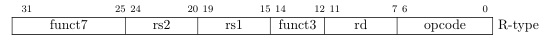
\includegraphics[scale=0.8]{figures/r_type.png}
    \caption{Fields in R-type instruction (source: RISC-V Instruction Set Manual)}
    \label{fig:Fields in R-type instruction}
\end{figure}
\pagebreak
\textbf{Extraction:}
\begin{figure}[H]
    \centering
    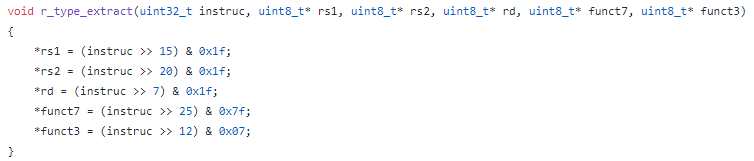
\includegraphics[scale=0.9]{figures/r_code.png}
    \caption{Extracting R type instruction}
    \label{fig:Extracting R type instruction}
\end{figure}

We illustrate the extraction of the value of \texttt{rd}, which is located in bits 8 to 12 in the instruction. In the above figure we see that to extract \texttt{rd} we first shifted the instruction to the right by 7 bits and used the bitwise AND operation with the bit mask \texttt{0x1f} to get the last five bits.\\
\\
\textbf{Binary format of instruction:} \texttt{0000 0000 1111 0111 0000 0111 1011 0011}\\
\textbf{Right shifted output:} \texttt{0000 0000 0000 0001 1110 1110 0000 1111}\\
\textbf{Output after masking:} \texttt{0000 0000 0000 0000 0000 0000 0000 1111}, which is 15.\\
We obtain the value of 15 for \texttt{rd} which is what we expect for the given instruction.
\\
\\

In the similar manner we extracted for other types of Instructions.
\newpage

\subsection{Execution of instructions}

After decoding the instruction and obtaining the required fields, we next implement the operation execution based on the instruction using C operators. First, the type of instruction is determined using the opcode. The opcode is obtained by performing the bitwise AND operation with the bit-mask \texttt{0x7f}. Then depending on the type of instruction, the appropriate operations are implemented.

\subsubsection{R-type instructions}
For these instruction we extract the values of \texttt{rs1}, \texttt{rs2}, \texttt{rd}, \texttt{funct3} and \texttt{funct7}. Here, based on the values of \texttt{funct3} and \texttt{funct7}, we operate on the values stored in register \texttt{rs1} and \texttt{rs2} and store the output in the location \texttt{rd}. For the unsigned instructions like \texttt{sltu} we cast the the value of the operands as unsigned integers using the inbuilt C casting operation.

\subsubsection{I-type instructions}
For the I-Type instructions, we extract the values of \texttt{rs1}, \texttt{rd}, \texttt{funct3} and \texttt{imm}. The exact operation is determined used the value of \texttt{funct3}.

\subsubsection{U-type instructions}
The instructions implemented here are AUIPC and LUI. The values of \texttt{rd} and \texttt{imm} are extracted for the computation. While LUI sets the lower 12bits of the \texttt{rd} register, AUIPC sets the \texttt{rd} to the appropriate address.

\subsubsection{Load instructions}
The Load instructions are encoded as I-Type instructions, and hence we extract the values of \texttt{rs1}, \texttt{rd}, \texttt{funct3} and \texttt{imm} in a similar fashion. The value stored in memory is extracted from the source address and stored in the target register after bit shifting and bit masking, according to the size (load word vs load half-word vs load byte)

\subsubsection{S-type instructions}
The store insturctions are encoded as S-type instructions, and we extract  \texttt{rs1}, \texttt{rs2}, \texttt{funct3} and \texttt{imm} fields. The correct destination in memory is calculated, and the value from the source register is stored in memory.

\subsubsection{J-type instructions}
The J-type instruction is used to implement the \texttt{jal} instruction. The \texttt{rd} and \texttt{imm} fields are read and an unconditional jump to the appropriate address is performed by adding the correct offset to the \texttt{pc}. The address of the next instruction after the jump is also written to the \texttt{rd} register.

\subsubsection{jalr instruction}
The \texttt{jalr} instruction is implemented as an I-type instruction, and hence \texttt{rs1}, \texttt{rd}, 
\texttt{funct3}, \texttt{imm} are extracted. The address of the next instruction following the current instruction is written to \texttt{rd}.

\subsubsection{B-type instruction}
The branch instructions are implemented as B-type instructions, and the appropriate fields \texttt{rs1}, \texttt{rs2}, \texttt{funct3}, and \texttt{imm} are extracted. Depending on the value of \texttt{funct3}, the appropriate type of branch instruction is chosen. The two source registers are compared and depending on the result of the operation, the appropriate address of the next instruction is written to the \texttt{pc} register. Note that the immediate values are expressed in multiples of 2 bytes, and hence this has to be accounted for while calculating the correct address for the next instruction.

\subsubsection{Environment Calls}
A few environment calls are also implemented:

\begin{tabular}{|c|c|c|}
\hline
     ID(a0)	& Name	& Description\\
     \hline
10&	\texttt{exit}&	Ends the program\\
1&	\texttt{print\_int}&	print intergers in a1\\
4&	\texttt{print\_string}&	prints the null-terminated string whose address is in a1\\
11&	\texttt{print\_character}&	prints ASCII character in a1\\
17&	\texttt{exit\_2}&	ends the program with return code in a1 \\
\hline
\end{tabular}

\subsection{Memory layout:}
\subsubsection{General purpose registers:}
In an actual RISC-V processor, general purpose registers are stored in the CPU. In order to simulate the same situation in the simulator, we allocated a separate space of 128 bytes other than the memory used for real memory operations.  
\subsubsection{Memory layout for program:}
In the simulator we allocated a total space of 32MB RAM for the microprocessor. We allocated memory for mainly text (or code), data and stack. The order of allocation would be i.e starting from address 0 to the text block. Data can be stored anywhere in the memory other than text or stack. Due to the large size of memory, there is very less possibility for collision and stack pointer is initialised to a high value to have sufficient space for stack.
\begin{figure}[H]
    \centering
    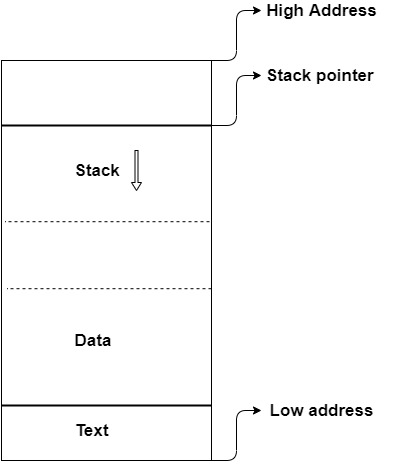
\includegraphics[scale=0.7]{figures/mem.jpg}
    \caption{Memory layout}
    \label{fig:Memory layout}
\end{figure}

\section{Building and running the simulator}
\newline To build the simulator, the \texttt{gcc-multilib} library is required, since the simulator is run as a 32-bit binary. Once the libary is installed, run \texttt{make}.\\
To run a binary file, type \texttt{./risc-simul <binary file>}\\
Any outputs, as well as the final register states are printed. A binary dump of the final register contents are also stored in \texttt{dump.res}






% PC operation\\
% Memory layout and stack pointer\\
% Description of files in submission folder\\
% Installation steps\\